\section{From event representations to multimodal measurement}
\label{sec:late}

The later experiments assembled spatial measurement, temporal transport, signed-TTC readout, and multimodal correction into one causal estimator. PHASE-TTC combines task adaptation and teacher supervision with event/RGB producers, context models, and a compact fusion head. No matched factorial separated all of these components, so the final result does not establish a JEPA contribution.

\subsection{V13: a parallel RGB route and a common temporal interface}

V13 added an RGB route with the event branch's A5, C2F, PAIR, and temporal-context decomposition. The common interface made it possible to test event information after an image-based TTC estimate. Each modality still used its own checkpoints, normalization, training data, and temporal support.

Three disjoint acquisition-group roles separated fitting stages. P supplied 53,890 queries from 24 sequences for producers and PAIR. H supplied 18,422 queries from eight sequences for downstream normalizers and heads, while V supplied 16,432 queries from eight sequences for internal evaluation. Earlier work had already used V, so its results remain development evidence.

PHASE17 connected both modalities to their context models through named phase, timing, and support fields. Their meanings remain stable across folds, whereas independently trained encoders can rotate their latent coordinates. The explicit interface enabled grouped out-of-fold training without a separate latent-alignment model.

\subsection{V14: changing the emphasis of the objective}

V14 could not improve short-TTC error without harming other ranges. Its six-cell factorial combined three sample-mass schemes with two losses, holding the frozen event producers, PAIR parent, and seed-7 draws fixed. Each 160-unit, two-layer GRU head received 2,500 updates over eight masked history slots and seventeen features; timestamps represented gaps without dense imputation.

M0 retained the native mass vector. M1 preserved mass per acquisition group while allocating TTC bands in the ratio 0.5/0.3/0.1/0.1. M2 also balanced crucial and long bands, bounding each row between 0.25 and four times its M1 weight. Uniform sampling with replacement kept the number of episodes unchanged. L0 retained the phase, quantile, and auxiliary objectives; L1 added
\begin{equation}
\mathcal L_1=\mathcal L_0+0.25\,\mathbb E_{i\sim\mathrm{batch}}
\left[Nm_i\,\mathrm{SmoothL1}\!\left(
\frac{\widehat T_i-T_i}{\max(|T_i|,0.5\,\mathrm{s})},0\right)\right],
\end{equation}
where $m_i$ is the registered sample mass. Both losses kept the native TTC mapping, clipping, and flat-gradient regions; neither used a straight-through estimator.

\begin{table}[tbp]
\centering\small
\caption{V14 factorial study on exposed V: apparent crucial-range gains can coexist with non-crucial regressions. Source \evidence{L02}.}
\label{tab:late_v14}
\begin{tabular}{lrrrr}
\toprule
\textbf{Model} & \textbf{MiD} & \textbf{Crucial} & \textbf{Negative} & \textbf{MAE (s)} \\
\midrule
RT-M0-L0-S7 & 106.21 & 156.83 & 61.38 & 2.51 \\
RT-M0-L1-S7 & 101.94 & 149.59 & 61.01 & 2.03 \\
RT-M1-L0-S7 & 102.23 & 134.47 & 84.21 & 2.98 \\
RT-M1-L1-S7 & 104.04 & 136.19 & 80.04 & 2.34 \\
RT-M2-L0-S7 & 104.32 & 134.87 & 87.62 & 3.37 \\
RT-M2-L1-S7 & 104.83 & 134.59 & 79.93 & 2.38 \\
\bottomrule
\end{tabular}
\end{table}

Every V14 candidate failed the full gate. M1--L0 reduced crucial-band MiD from 156.8 to 134.5, while large-band error rose from 52.2 to 76.4 and negative-band error from 61.4 to 84.2. M0--L1 achieved the best aggregate and MAE in the matrix, but missed the required crucial-band improvement and other safeguards. All outputs were finite; the failures came from measured regressions. \evidence{L02}

Only 76 V queries fell in the urgent interval $(0.1,1]$ seconds. Across the factorial, 81.6--100\% received late warnings; negative TTC predictions did not count as positive warnings. Such miss rates preclude a safety claim regardless of false-alert rate.

V14 closed as \texttt{NO\_CANDIDATE}, so the conditional replication and transfer stages did not run. The factorial exposed a tradeoff between urgent-range accuracy and the other signed-TTC ranges without producing an admissible improvement.

\begin{figure}[t]
\centering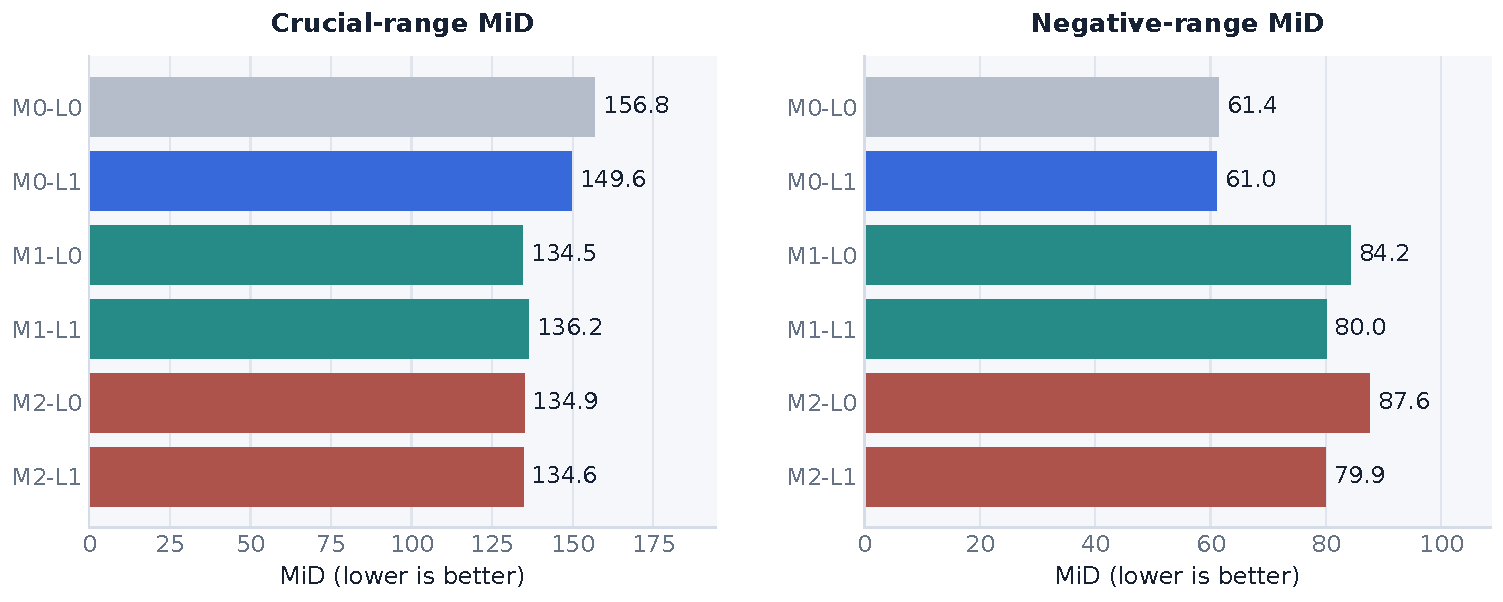
\includegraphics[width=0.98\linewidth]{figures/range_tradeoffs.pdf}
\caption{V14 MiD changes across crucial, small, large, and negative TTC bands.}
\end{figure}

\subsection{V15 and V17: testing readout and geometry explanations}

Neither V15 intervention passed all gates. Sampling proportional to sample mass, corrected by $w_i/p_i$, preserved V14's cross-band tradeoff. Expanding the A5 residual range through an equal-slope hyperbolic tangent left crucial-band performance almost unchanged. The modified producer received regenerated PHASE17 fields and H normalizers.

V17 tested frozen geometry from several angles. A bypass exposed geometry and transport tokens to the temporal head; other arms examined learned NLL precision, grouped ridge probes, directional differences, height calibration and supervision, vertical position, gradient clipping, and nonlinear spatial-height readout. Each had a dedicated control. Directional differences remove static levels while also reducing dimensionality, so they do not isolate appearance memorization.

The geometry bypass carried a useful but unstable downstream signal. On V, its three-seed mean improved crucial MiD from 157.1 to 148.4 and aggregate MiD from 106.5 to 102.8, while MAE worsened. The effect was stronger on H than V, and the three heads shared encoders rather than repeating representation training. \evidence{L50}

The first height-regression arm emitted predictions outside the admissible MiD domain. We kept those rows and left its aggregate missing instead of clipping them away. Temporal supervision restored coverage but not competitive TTC accuracy. Preserving vertical positions improved training height fit while worsening H TTC, and the nonlinear readout also failed. The tested frozen-feature calibration was insufficient, though the bypass result still showed usable geometric signal.

Removing gradient clipping changed little. Learned precision improved crucial-band error in every head seed, but missed the required magnitude and safeguards. The recorded gradient norms describe one loss component rather than the full-dataset objective. None of V17's nine research lines produced a candidate. \evidence{L51,L52}

\subsection{V18: adaptation of the measurement stage}

V18 moved adaptation into the measurement stage. Its primary comparison covered direct and correspondence-based pair readouts, trained and frozen encoders, and a native-system control. C1 tested geometric readout, D1 predictor width, B1 auxiliary correspondence supervision, and A1 adaptation depth. Some arms also updated correspondence, so equal TTC-update counts did not mean equal computation.

C1 improved bandwise geometry over an unconstrained pair-correction readout but failed as a complete TTC estimator. D1 found no benefit from greater predictor width. B1 beat a TTC-only control at the same number of TTC updates, yet its negative-band error blocked promotion over A5. A1 then compared full adaptation with partial retention of the correspondence-trained representation.

A1-FULL delivered V18's largest TTC gain and its clearest tradeoff. On H, aggregate MiD fell from 112.3 for A5-P2 to 78.9, and crucial MiD from 157.3 to 95.8; negative MiD rose from 65.5 to 87.1. It passed the global sign-error safeguard and beat last-block adaptation overall, but did not preserve accurate negative magnitude or demonstrate retention of the correspondence representation. \evidence{L10,L24,L25}

C1 also tested event information after the RGB context estimate. TRUE fusion and an equal-capacity ZERO-event control used seeds 7, 13, and 23. Each seed repeated C1 adaptation and head fitting, while all shared the historical A5 initialization and RGB context parent. The comparison isolates event input within this configuration, not variability from complete pretraining.

TRUE fusion improved on ZERO within V18. Across seeds, aggregate MiD was $87.3\pm0.9$ for TRUE and $92.5\pm0.2$ for ZERO; TRUE's crucial MiD was $126.6\pm0.9$. A paired whole-group bootstrap favored TRUE in aggregate loss. The crucial-band gain missed the preregistered 10\% threshold, and the interval against the preserved V16 PHASE-ONLY family crossed zero at about $[-3.7,0.1]$. Thus, events complemented RGB in this model without establishing superiority over V16. \evidence{L03,L31,L32,L33}

No V18 arm satisfied the complete promotion gate, and the campaign closed as \texttt{NO\_CANDIDATE}. A later portability replay verified archived metrics and exports without adding training or performance evidence.

\begin{table}[tbp]
\centering\small
\caption{V18 primary and adaptive experiments on development subset H (18,422 rows). Sources \evidence{L10--L14,L20--L25}.}
\label{tab:late_v18}
\begin{tabular}{lrrrr}
\toprule
\textbf{Model} & \textbf{MiD} & \textbf{Crucial} & \textbf{Negative} & \textbf{MAE (s)} \\
\midrule
A5-P2-FROZEN & 112.29 & 157.27 & 65.52 & 5.64 \\
PAIR-DIRECT-S7 & 103.87 & 117.98 & 148.17 & 5.00 \\
PAIR-CORR-S7 & 103.51 & 115.56 & 156.00 & 5.50 \\
PAIR-CORR-FROZEN-S7 & 106.72 & 123.61 & 146.99 & 5.40 \\
NATIVE-P2-FT-S7 & 104.05 & 145.12 & 61.26 & 4.65 \\
PAIR-CORR-GEOMETRY-S7 & 90.95 & 114.35 & 106.23 & 6.95 \\
PAIR-CORR-WIDE-S7 & 115.12 & 124.48 & 206.42 & 6.79 \\
B1-TTC-CONTROL-STAGE2-S7 & 85.98 & 106.71 & 96.63 & 6.11 \\
B1-CORRESPONDENCE-STAGE2-S7 & 81.44 & 100.22 & 84.12 & 5.48 \\
A1-LAST-BLOCK-S7 & 90.64 & 111.03 & 97.96 & 7.11 \\
A1-FULL-S7 & 78.92 & 95.85 & 87.09 & 5.45 \\
\bottomrule
\end{tabular}
\end{table}
\begin{table}[tbp]
\centering\small
\caption{V18 C1 equal-capacity TRUE/ZERO event controls on exposed V (16,432 rows), using adaptation/head seeds 7, 13, and 23. Source \evidence{L03}.}
\label{tab:late-fusion}
\begin{tabular}{lrrr}
\toprule
\textbf{Head / seed} & \textbf{Overall MiD} & \textbf{Crucial MiD} & \textbf{MAE (s)} \\
\midrule
FUSION-TRUE-S7 & 88.270 & 127.661 & 1.817 \\
FUSION-ZERO-S7 & 92.638 & 136.989 & 1.842 \\
FUSION-TRUE-S13 & 86.630 & 125.976 & 1.807 \\
FUSION-ZERO-S13 & 92.455 & 136.500 & 1.837 \\
FUSION-TRUE-S23 & 86.961 & 126.069 & 1.818 \\
FUSION-ZERO-S23 & 92.315 & 136.314 & 1.836 \\
\bottomrule
\end{tabular}
\end{table}
\begin{figure}[t]
\centering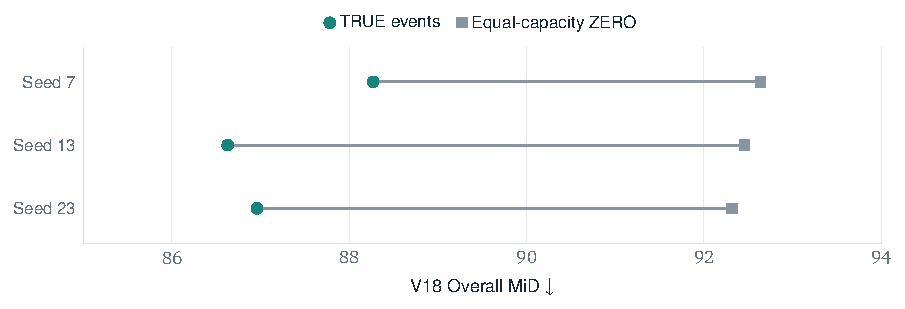
\includegraphics[width=0.98\linewidth]{figures/rev_v18.pdf}
\caption{V18 measurement adaptations and paired TRUE/ZERO event-fusion controls.}
\end{figure}

\subsection{V19: repairing negative motion changes the tradeoff}

V19 tested loss weighting as the source of A1's negative-band regression. L0 and LW shared the correspondence-trained B1 parent, full adaptation, seed 7, uniform sampling, and 12,000 updates. L0 assigned crucial/small/large/negative masses of 50/30/10/10\%. LW doubled negative mass to 20\% and set the positive bands to 44.44/26.67/8.89\%, preserving their relative proportions. The encoder did not change.

\begin{table}[tbp]
\centering\small
\caption{V19 decision recovery on exposed H. LW trades a small overall MiD increase against improved MAE and negative-range behavior. Source \evidence{L30}.}
\label{tab:late_v19}
\begin{tabular}{lrrrr}
\toprule
\textbf{Model} & \textbf{MiD} & \textbf{Crucial} & \textbf{Negative} & \textbf{MAE (s)} \\
\midrule
A5 & 112.29 & 157.27 & 65.52 & 5.64 \\
L0 & 78.92 & 95.85 & 87.09 & 5.45 \\
LW & 79.87 & 100.42 & 70.78 & 4.61 \\
\bottomrule
\end{tabular}
\end{table}

LW repaired part of the negative-motion error but worsened the primary aggregate. Relative to L0, it reduced negative MiD by 18.7\%, MAE by 15.3\%, and sign error by 1.55 percentage points, while aggregate and crucial MiD increased. The same pattern appeared on P training data, ruling out an H-only generalization failure. Because the replication trigger required lower aggregate error, LW did not advance. \evidence{L30}

Later two-expert selectors also failed the system gate. They required both fitted experts and the measured feature path, rather than forming a jointly trained sparse mixture. Grouped validation limited fitting leakage, while reused H data and fixed experts constrained the conclusion to these selectors.
\FloatBarrier
